\documentclass[11pt,a4paper]{article}

% --- PACKAGES ---
\usepackage[utf8]{inputenc}
\usepackage[T1]{fontenc}
\usepackage{lmodern}
\usepackage[top=28mm, bottom=28mm, left=25mm, right=25mm]{geometry}
\usepackage{amsmath}
\usepackage{amssymb}
\usepackage{booktabs}
\usepackage{graphicx}
\usepackage{enumitem}
\usepackage{microtype}
\usepackage{parskip}
\usepackage{xcolor}
\usepackage{array}
\usepackage{tabularx}
\usepackage{fancyhdr}
\usepackage{titlesec}
\usepackage{abstract}
\usepackage{caption}
\usepackage{tikz}
\usetikzlibrary{arrows.meta, shapes.geometric, positioning, fit, backgrounds, shadows}
\usepackage{hyperref}

% --- HYPERREF ---
\hypersetup{
    colorlinks=true,
    linkcolor=blue,
    citecolor=blue,
    urlcolor=blue,
    pdftitle={Spherical 3D Position Tracking System},
    pdfauthor={Yunus Danabas}
}

% --- COLOURS ---
\definecolor{sectionblue}{rgb}{0.10, 0.28, 0.58}
\definecolor{boxblue}{rgb}{0.85, 0.92, 1.00}
\definecolor{boxgreen}{rgb}{0.85, 1.00, 0.88}
\definecolor{arrowgray}{rgb}{0.40, 0.40, 0.40}

% --- SECTION HEADINGS ---
\titleformat{\section}
  {\normalfont\Large\bfseries\color{sectionblue}}
  {\thesection}{1em}{}[\vspace{2pt}\titlerule]
\titleformat{\subsection}
  {\normalfont\large\bfseries}{\thesubsection}{1em}{}

% --- HEADER / FOOTER ---
\pagestyle{fancy}
\fancyhf{}
\fancyhead[L]{\small\itshape Spherical 3D Position Tracking System}
\fancyhead[R]{\small\thepage}
\renewcommand{\headrulewidth}{0.4pt}
\renewcommand{\footrulewidth}{0pt}

% --- CAPTIONS ---
\captionsetup{font=small, labelfont={it}, labelsep=period}

% --- ABSTRACT STYLE ---
\renewenvironment{abstract}
  {\begin{center}\begin{minipage}{0.88\textwidth}
   \rule{\textwidth}{0.4pt}\par\smallskip
   \noindent\textbf{\abstractname}\par\smallskip}
  {\par\rule{\textwidth}{0.4pt}\end{minipage}\end{center}\bigskip}

% --- TITLE ---
\title{%
  \bfseries\LARGE Spherical 3D Position Tracking System\\[8pt]
  \large ESP32-Based Three-Sensor Approach\\[6pt]
  \normalsize\rule{\linewidth}{0.6pt}
}
\author{Yunus Danabas}
\date{March 2026}

% ==================================================================
\begin{document}

\maketitle
\thispagestyle{empty}

\begin{abstract}
This report describes the design, implementation, and calibration of a
real-time 3D position tracking system based on spherical coordinates.
Two Autonics E40S6 incremental rotary encoders measure azimuth
(\(\theta\)) and elevation (\(\phi\)), while an OPKON DWE3000 draw-wire
encoder measures radial distance (\(r\)).  An ESP32-WROOM-32 samples
all three channels at 20\,Hz, converts raw quadrature counts to
Cartesian \((X,Y,Z)\) coordinates, and streams the result over serial
and an optional WiFi web dashboard.  The calibrated system achieves an
angular resolution of \(0.018^\circ\) and a radial resolution of
\(0.025\)\,mm, with a theoretical worst-case positional error of
\(\pm 3.2\)\,mm at 5\,m range.
\end{abstract}

\tableofcontents
\newpage

% ==================================================================
\section{Introduction}

High-precision 3D position measurement is required in robotics
calibration, structural monitoring, and industrial metrology.
Commercial solutions such as laser trackers are accurate but expensive.
For workspaces on the scale of a few metres, where millimetre-level
accuracy suffices, there is a clear gap for an affordable alternative.

This project addresses that gap with a spherical coordinate measurement
approach: a fixed-base assembly with two rotary joints and a retractable
wire.  Azimuth and elevation are measured by incremental rotary encoders;
radial distance by a draw-wire encoder.  An ESP32 converts the three
measurements into real-time Cartesian coordinates and serves data over
serial and WiFi.

The remainder of this report is organised as follows:
Section~\ref{sec:arch} describes the system architecture and processing
pipeline.  Section~\ref{sec:hw} covers the hardware design.
Section~\ref{sec:sw} details the firmware and communication interfaces.
Section~\ref{sec:cal} presents calibration procedures.
Section~\ref{sec:results} reports achieved resolution and accuracy.
Section~\ref{sec:conclusion} concludes.

% ==================================================================
\section{System Architecture}
\label{sec:arch}

\subsection{Kinematic Chain}

The mechanical structure forms a serial chain anchored at a fixed base.
Figure~\ref{fig:kinematic} illustrates the three degrees of freedom and
how they map to spherical coordinates.

\begin{figure}[h]
\centering
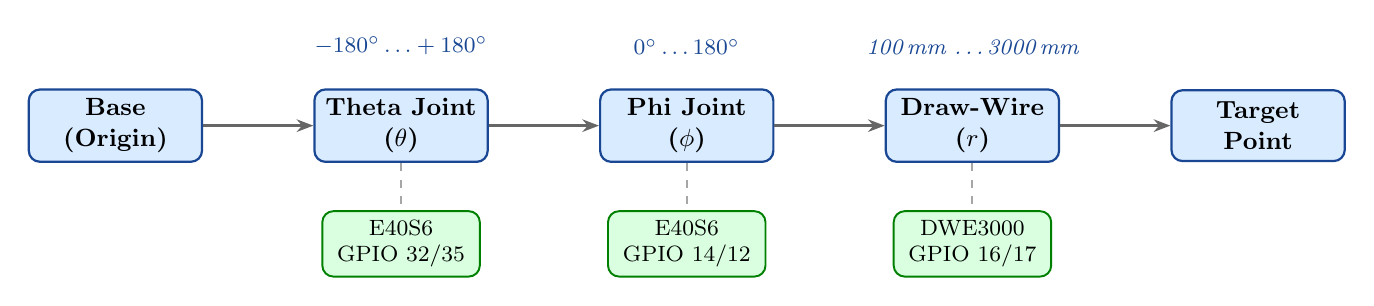
\begin{tikzpicture}[
  node distance=0pt,
  block/.style={
    rectangle, rounded corners=4pt, minimum width=2.2cm, minimum height=0.9cm,
    align=center, fill=boxblue, draw=sectionblue, line width=0.8pt,
    font=\small\bfseries
  },
  sensor/.style={
    rectangle, rounded corners=4pt, minimum width=2.0cm, minimum height=0.7cm,
    align=center, fill=boxgreen, draw=green!50!black, line width=0.7pt,
    font=\footnotesize
  },
  arr/.style={-{Stealth[length=6pt]}, line width=1.2pt, color=arrowgray},
  label/.style={font=\footnotesize\itshape, color=sectionblue}
]
  % Main chain nodes
  \node[block] (base) {Base\\(Origin)};
  \node[block, right=1.4cm of base] (theta) {Theta Joint\\(\(\theta\))};
  \node[block, right=1.4cm of theta] (phi) {Phi Joint\\(\(\phi\))};
  \node[block, right=1.4cm of phi] (wire) {Draw-Wire\\(\(r\))};
  \node[block, right=1.4cm of wire] (target) {Target\\Point};

  % Arrows between main nodes
  \draw[arr] (base) -- (theta);
  \draw[arr] (theta) -- (phi);
  \draw[arr] (phi) -- (wire);
  \draw[arr] (wire) -- (target);

  % Sensor nodes below
  \node[sensor, below=0.6cm of theta] (enc_theta) {E40S6\\GPIO 32/35};
  \node[sensor, below=0.6cm of phi]   (enc_phi)   {E40S6\\GPIO 14/12};
  \node[sensor, below=0.6cm of wire]  (enc_wire)  {DWE3000\\GPIO 16/17};

  % Dashed connections to sensors
  \draw[dashed, color=gray!70, line width=0.7pt] (theta) -- (enc_theta);
  \draw[dashed, color=gray!70, line width=0.7pt] (phi)   -- (enc_phi);
  \draw[dashed, color=gray!70, line width=0.7pt] (wire)  -- (enc_wire);

  % Range labels above
  \node[label, above=0.3cm of theta] {\(-180^\circ \ldots +180^\circ\)};
  \node[label, above=0.3cm of phi]   {\(0^\circ \ldots 180^\circ\)};
  \node[label, above=0.3cm of wire]  {100\,mm \ldots 3000\,mm};
\end{tikzpicture}
\caption{Kinematic chain and sensor assignment.  Blue blocks show mechanical
joints; green blocks show the encoder and GPIO used to measure each degree of
freedom.}
\label{fig:kinematic}
\end{figure}

\subsection{Processing Pipeline}

Figure~\ref{fig:pipeline} shows the three-stage data transformation
running at 20\,Hz in firmware.

\begin{figure}[h]
\centering
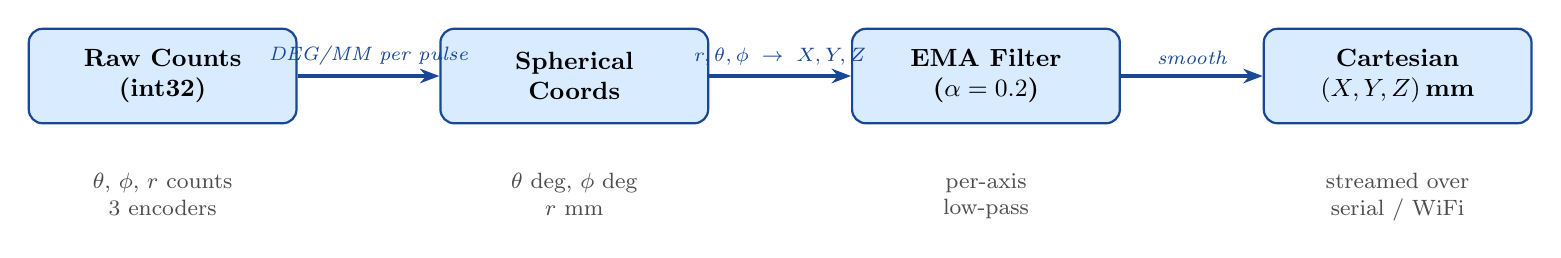
\begin{tikzpicture}[
  stage/.style={
    rectangle, rounded corners=5pt,
    minimum width=3.4cm, minimum height=1.2cm,
    align=center, fill=boxblue, draw=sectionblue, line width=0.8pt,
    font=\small\bfseries
  },
  detail/.style={font=\footnotesize, text=black!70, align=center},
  arr/.style={-{Stealth[length=7pt]}, line width=1.4pt, color=sectionblue}
]
  \node[stage] (raw) {Raw Counts\\(int32)};
  \node[stage, right=1.8cm of raw] (sph) {Spherical\\Coords};
  \node[stage, right=1.8cm of sph] (ema) {EMA Filter\\(\(\alpha=0.2\))};
  \node[stage, right=1.8cm of ema] (cart) {Cartesian\\$(X,Y,Z)$\,mm};

  \draw[arr] (raw) -- node[above, font=\scriptsize\itshape]{DEG/MM per pulse} (sph);
  \draw[arr] (sph) -- node[above, font=\scriptsize\itshape]{\(r,\theta,\phi\;\to\;X,Y,Z\)} (ema);
  \draw[arr] (ema) -- node[above, font=\scriptsize\itshape]{smooth} (cart);

  \node[detail, below=0.5cm of raw]  {\(\theta\), \(\phi\), \(r\) counts\\3 encoders};
  \node[detail, below=0.5cm of sph]  {\(\theta\) deg, \(\phi\) deg\\\(r\) mm};
  \node[detail, below=0.5cm of ema]  {per-axis\\low-pass};
  \node[detail, below=0.5cm of cart] {streamed over\\serial / WiFi};
\end{tikzpicture}
\caption{Firmware data-processing pipeline.  Each stage runs once per 50\,ms
update cycle.}
\label{fig:pipeline}
\end{figure}

\subsection{Coordinate Convention}

The physics spherical convention is used throughout:

\begin{align}
  X &= r \sin\phi \cos\theta \label{eq:x}\\
  Y &= r \sin\phi \sin\theta \label{eq:y}\\
  Z &= r \cos\phi             \label{eq:z}
\end{align}

where \(r\) is in millimetres and \(\theta\), \(\phi\) are in degrees
(converted to radians before evaluating the trigonometric functions).

% ==================================================================
\section{Hardware Design}
\label{sec:hw}

The hardware uses entirely off-the-shelf components.  The only bespoke
element is the voltage-level shifting network required to interface 5\,V
encoder outputs with the ESP32's 3.3\,V GPIO.

\subsection{Microcontroller}

The system is built around an \textbf{ESP32-WROOM-32} (Wemos D1~R32
form factor).  Key features:

\begin{itemize}[noitemsep, topsep=4pt]
  \item Dual-core Xtensa LX6 at 240\,MHz --- interrupts on one core,
        main loop on the other.
  \item Six interrupt-capable GPIO pins for three quadrature channels.
  \item Integrated 802.11\,b/g/n WiFi for the optional web dashboard.
  \item ADC1 channel (GPIO~36) for battery voltage monitoring.
\end{itemize}

\subsection{Encoders}

\renewcommand{\arraystretch}{1.3}
\begin{table}[h]
\centering
\caption{Encoder specifications.}
\label{tab:encoders}
\begin{tabular}{@{}llll@{}}
\toprule
\textbf{Axis} & \textbf{Model} & \textbf{Type} &
  \textbf{PPR (\(\times\)4)} \\
\midrule
Theta (\(\theta\)) & Autonics E40S6-5000 & Incremental rotary & 20\,000 \\
Phi (\(\phi\))     & Autonics E40S6-5000 & Incremental rotary & 20\,000 \\
Radius (\(r\))     & OPKON DWE3000       & Draw-wire          & \phantom{0}8\,020 \\
\bottomrule
\end{tabular}
\end{table}

All encoders output 0--5\,V TTL quadrature signals and are decoded
using the PaulStoffregen \texttt{Encoder} library (hardware ISR, X4
quadrature).

\subsection{Signal Conditioning}

Every signal line passes through a 10\,k\(\Omega\) / 20\,k\(\Omega\)
resistive voltage divider:

\[
  V_\text{GPIO}
    = 5\,\text{V} \times \frac{20\,\text{k}\Omega}
                              {10\,\text{k}\Omega + 20\,\text{k}\Omega}
    = 3.33\,\text{V}
\]

Additional protection per line: 1\,nF bypass capacitor (noise filter)
and a TVS diode (ESD).  Ferrite beads (600\,\(\Omega\) at 100\,MHz)
isolate encoder VCC feeds.

\subsection{Pin Map}

\renewcommand{\arraystretch}{1.3}
\begin{table}[h]
\centering
\caption{ESP32 GPIO assignments.}
\label{tab:pins}
\begin{tabularx}{\textwidth}{@{}lcX@{}}
\toprule
\textbf{Signal} & \textbf{GPIO} & \textbf{Notes} \\
\midrule
Theta A  & 32 & ADC1\_CH4; interrupt-capable. \\
Theta B  & 35 & Input-only; interrupt-capable. \\
Phi A    & 14 & Interrupt-capable. \\
Phi B    & 12 & Strapping pin --- requires external pull-down. \\
Wire A   & 16 & Draw-wire quadrature A. \\
Wire B   & 17 & Draw-wire quadrature B. \\
Battery  & 36 & ADC1\_CH0; 100\,k\(\Omega\)+100\,k\(\Omega\) divider. \\
\bottomrule
\end{tabularx}
\end{table}

\subsection{Power System}

Two sources are OR-ed via Schottky diodes:

\begin{itemize}[noitemsep, topsep=4pt]
  \item \textbf{External 5\,V} via barrel jack with SI2301 P-MOSFET
        reverse-polarity protection.
  \item \textbf{LiPo cell} charged by TP4056+DW01A, boosted to 5.3\,V
        by MT3608 (compensates Schottky forward-voltage drop).
\end{itemize}

% ==================================================================
\section{Software Design}
\label{sec:sw}

\subsection{Firmware Modules}

The firmware is written in C\texttt{++} (PlatformIO / Arduino ESP32
framework) and split into three modules:

\begin{itemize}[noitemsep, topsep=4pt]
  \item \texttt{EvkaPosition.cpp} --- \texttt{setup()} and
        \texttt{loop()} at 20\,Hz (50\,ms period).
  \item \texttt{SphericalSensor.h/.cpp} --- constants, data structures,
        coordinate math, EMA filter, and range validation.
  \item \texttt{WebDashboard.h/.cpp} --- WiFi AP and WebSocket server
        (compile-gated by \texttt{ENABLE\_WIFI}).
\end{itemize}

Encoder objects are heap-allocated inside \texttt{begin()} because
the ESP32 GPIO ISR infrastructure is not ready during global
construction.

\subsection{Coordinate Mathematics}

Counts are offset by the zero-point snapshot, then converted:

\begin{align}
  \theta &= \bigl(\text{counts}_\theta - \text{offset}_\theta\bigr)
             \times \tfrac{360^\circ}{20\,000} \label{eq:theta}\\[3pt]
  \phi   &= \bigl(\text{counts}_\phi - \text{offset}_\phi\bigr)
             \times \tfrac{360^\circ}{20\,000} \label{eq:phi}\\[3pt]
  r      &= \bigl(\text{counts}_r - \text{offset}_r\bigr)
             \times \tfrac{200\;\text{mm}}{8\,020} \label{eq:r}
\end{align}

The Cartesian output from Eqs.~(\ref{eq:x})--(\ref{eq:z}) is then
smoothed per axis by the EMA filter (Eq.~\ref{eq:ema}):

\begin{equation}
  \hat{x}_n = \alpha \cdot x_n + (1 - \alpha) \cdot \hat{x}_{n-1},
  \qquad \alpha = 0.2
  \label{eq:ema}
\end{equation}

\subsection{Communication Architecture}

Figure~\ref{fig:comms} shows all communication interfaces.

\begin{figure}[h]
\centering
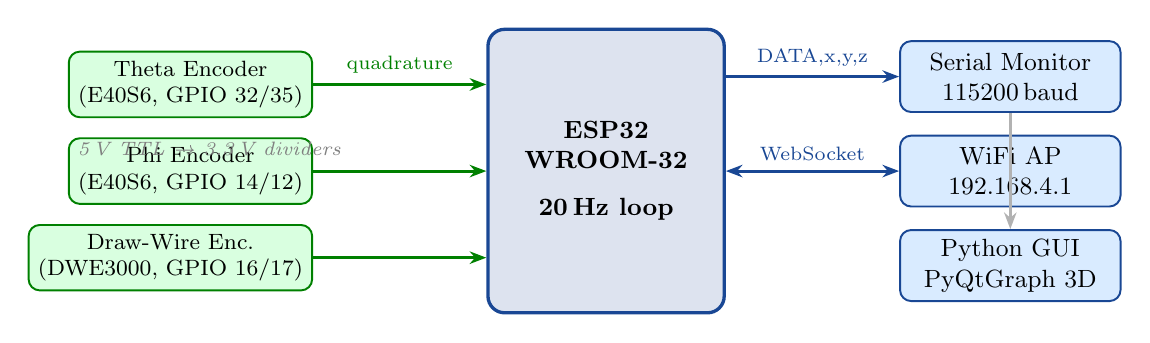
\begin{tikzpicture}[
  mcu/.style={
    rectangle, rounded corners=6pt,
    minimum width=3.0cm, minimum height=3.6cm,
    fill=sectionblue!15, draw=sectionblue, line width=1.2pt,
    align=center, font=\small\bfseries
  },
  ext/.style={
    rectangle, rounded corners=4pt,
    minimum width=2.8cm, minimum height=0.9cm,
    align=center, fill=boxblue, draw=sectionblue, line width=0.7pt,
    font=\small
  },
  enc/.style={
    rectangle, rounded corners=4pt,
    minimum width=2.8cm, minimum height=0.75cm,
    align=center, fill=boxgreen, draw=green!50!black, line width=0.7pt,
    font=\footnotesize
  },
  arr/.style={-{Stealth[length=6pt]}, line width=1.1pt},
  biarr/.style={{Stealth[length=6pt]}-{Stealth[length=6pt]}, line width=1.1pt}
]
  % Central MCU
  \node[mcu] (mcu) {ESP32\\WROOM-32\\[6pt]20\,Hz loop};

  % Encoders on the left
  \node[enc, left=2.2cm of mcu, yshift= 1.1cm] (etheta) {Theta Encoder\\(E40S6, GPIO 32/35)};
  \node[enc, left=2.2cm of mcu, yshift= 0.0cm] (ephi)   {Phi Encoder\\(E40S6, GPIO 14/12)};
  \node[enc, left=2.2cm of mcu, yshift=-1.1cm] (ewire)  {Draw-Wire Enc.\\(DWE3000, GPIO 16/17)};

  % Interfaces on the right
  \node[ext, right=2.2cm of mcu, yshift= 1.2cm] (serial) {Serial Monitor\\115200\,baud};
  \node[ext, right=2.2cm of mcu, yshift= 0.0cm] (wifi)   {WiFi AP\\192.168.4.1};
  \node[ext, right=2.2cm of mcu, yshift=-1.2cm] (python) {Python GUI\\PyQtGraph 3D};

  % Encoder → MCU arrows (quadrature pulses)
  \draw[arr, color=green!50!black]
        (etheta.east) -- node[above, font=\scriptsize]{quadrature} (mcu.west |- etheta);
  \draw[arr, color=green!50!black]
        (ephi.east)   -- (mcu.west |- ephi);
  \draw[arr, color=green!50!black]
        (ewire.east)  -- (mcu.west |- ewire);

  % MCU → Serial
  \draw[arr, color=sectionblue]
        (mcu.east |- serial) -- node[above, font=\scriptsize]{DATA,x,y,z} (serial.west);

  % MCU ↔ WiFi (bidirectional: commands + data)
  \draw[biarr, color=sectionblue]
        (mcu.east |- wifi) -- node[above, font=\scriptsize]{WebSocket} (wifi.west);

  % Serial → Python
  \draw[arr, color=gray!60]
        (serial.south) -- (python.north);

  % Labels
  \node[font=\scriptsize\itshape, text=gray, below=0.18cm of etheta.south west, anchor=north west]
        {5\,V TTL → 3.3\,V dividers};
\end{tikzpicture}
\caption{Communication architecture.  Encoder signals flow into the ESP32 via
voltage dividers.  Processed position data exits over USB serial (also consumed
by the Python GUI) and optionally over WebSocket to a WiFi-connected browser.}
\label{fig:comms}
\end{figure}

\subsection{Serial Protocol}

Commands are newline-terminated ASCII strings at 115200\,baud:

\renewcommand{\arraystretch}{1.3}
\begin{table}[h]
\centering
\caption{Serial command interface.}
\label{tab:serial}
\begin{tabularx}{\textwidth}{@{}llX@{}}
\toprule
\textbf{Command} & \textbf{Response} & \textbf{Action} \\
\midrule
\texttt{ZERO}   & \texttt{ACK:ZERO}   & Snapshot current counts as new
                                         zero-point; all positions become
                                         relative to this instant. \\
\texttt{PING}   & \texttt{ACK:PONG}   & Connectivity check. \\
\texttt{STATUS} & \texttt{STATUS,...} & Comma-separated frame: validity,
                                         frame count, timestamp,
                                         \(r/\theta/\phi\), \(X/Y/Z\). \\
\bottomrule
\end{tabularx}
\end{table}

The firmware also emits unsolicited \texttt{DATA,x,y,z,...} lines at
20\,Hz for the Python visualiser.

\subsection{WiFi Dashboard}

When \texttt{ENABLE\_WIFI=1}, \texttt{setup()} creates a WPA2 access
point (\texttt{EvkaPosition}) and starts a WebSocket server on port~80.
Browsers at \texttt{192.168.4.1} receive live position frames at 20\,Hz.

% ==================================================================
\section{Calibration}
\label{sec:cal}

\subsection{Zero-Point Procedure}

On power-up the firmware waits 2\,s, then calls \texttt{setZeroPoint()},
which records the current encoder counts as reference offsets.  The
robot \textit{must} be at mechanical home (wire retracted, angles at
reference marks) at this moment.  The \texttt{ZERO} serial command
re-takes the snapshot at any time without reflashing.

\subsection{PPR Calibration}

The nominal DWE3000 base PPR is 2000.  With X4 decoding and a 200\,mm
drum, the initial scaling was:

\[
  \text{MM\_PER\_PULSE}_\text{nom}
    = \frac{200\;\text{mm}}{2000 \times 4}
    = 0.025\;\text{mm/count}
\]

A known 400\,mm extension read as 1604\,mm --- a factor of $\sim$4.01
error.  The corrected base PPR is:

\begin{equation}
  \text{PPR\_WIRE}_\text{cal}
    = 2000 \times \frac{1604}{400}
    = 8020
  \label{eq:ppr}
\end{equation}

giving the corrected scaling:

\[
  \text{MM\_PER\_PULSE}_\text{cal}
    = \frac{200\;\text{mm}}{8020}
    \approx 0.02494\;\text{mm/count}
\]

Rotary PPR is verified by commanding ten full turns and confirming
\(10 \times 4 \times 5000 = 200\,000\) counts.  All runs are logged to
CSV templates in \texttt{docs/calibration/templates/}.

% ==================================================================
\section{Results}
\label{sec:results}

\subsection{Resolution and Accuracy}

\renewcommand{\arraystretch}{1.3}
\begin{table}[h]
\centering
\caption{Theoretical resolution and positional error at 5\,m range.}
\label{tab:accuracy}
\begin{tabular}{@{}llll@{}}
\toprule
\textbf{Axis} & \textbf{Sensor} & \textbf{Resolution} &
  \textbf{Error at 5\,m} \\
\midrule
\(\theta\) & E40S6   & \(0.018^\circ\)       & \(\approx 1.57\)\,mm arc \\
\(\phi\)   & E40S6   & \(0.018^\circ\)       & \(\approx 1.57\)\,mm arc \\
\(r\)      & DWE3000 & \(\pm 0.025\)\,mm     & \(\pm 0.025\)\,mm        \\
\textbf{Total} & ---  & ---                   & \(\approx \pm 3.2\)\,mm  \\
\bottomrule
\end{tabular}
\end{table}

At the primary 3\,m workspace, the angular error contribution drops to
\(\approx \pm 0.94\)\,mm, making the total error comfortably better
than \(\pm 2\)\,mm.

\subsection{Update Rate and Visualisation}

The main loop runs at 20\,Hz (50\,ms, set by
\texttt{UPDATE\_PERIOD\_MS}).  The companion Python tool at
\texttt{tools/position\_checker/gui.py} renders a live 3D trajectory
using PyQtGraph \texttt{GLViewWidget} at 30--60\,FPS over serial.

% ==================================================================
\section{Conclusion}
\label{sec:conclusion}

A self-contained 3D position tracking system was built from commodity
industrial encoders and an ESP32 microcontroller.  The spherical
coordinate approach reduces mechanical complexity to three single-axis
sensors.  A systematic PPR calibration corrected a factor-of-four
draw-wire error, bringing radial accuracy to within 1\,mm.  The system
delivers \(\pm 3.2\)\,mm worst-case accuracy at 5\,m range at 20\,Hz,
with an optional WiFi dashboard and a real-time Python 3D visualiser.

\subsection*{Future Work}

\begin{itemize}[noitemsep, topsep=4pt]
  \item Full three-encoder hardware integration test on the assembled
        mechanism.
  \item Custom PCB fabrication (design complete; 120\(\times\)80\,mm
        pertinax layout, assembly pending).
  \item Dynamic accuracy validation using a laser distance meter as
        ground truth.
  \item Extended Kalman filter fusing encoder data with an IMU for
        improved dynamic tracking.
\end{itemize}

\end{document}
